%% Migrated from the MICCAI/LNCS manuscript to Elsevier's CAS
%% double-column format for submission to Information Fusion.
\documentclass[a4paper,fleqn]{cas-dc}

\usepackage[T1]{fontenc}
\usepackage[numbers]{natbib}
\usepackage{amsmath}
\usepackage{amssymb}
\usepackage{graphicx}
\usepackage{booktabs}
\usepackage{microtype}
\microtypesetup{expansion=false}
\definecolor{CERDblue}{HTML}{4C78A8}
\definecolor{CERDorange}{HTML}{D97732}

% Keep table typography consistent with the serif body text. The CAS class
% switches tables and their captions to sans serif by default.
\AtBeginEnvironment{tabular}{\rmfamily}
\AtBeginEnvironment{tabular*}{\rmfamily}
\ExplSyntaxOn
\patchcmd{\__make_tbl_caption:nn}
  {\sffamily\small}
  {\rmfamily\small}
  {}{}
% Use the manuscript's serif text face for running heads and figure captions;
% the CAS defaults use a contrasting sans-serif face.
\cs_set:Npn \__cas_head:
{
  \parbox{\textwidth}
  {
    \rmfamily\small\centering
    \__short_title:
  }
}
\cs_set_eq:cc { @oddhead } { __cas_head: }
\cs_set_eq:cc { @evenhead } { __cas_head: }
\cs_set:Npn \__make_fig_caption:nn #1#2
{
  \l_fig_align_tl
  \skip_vertical:N \l_fig_abovecap_skip
  \setbox\cascaptionbox=\hbox{%
    \rmfamily\small\textbf{\color{scolor}#1:}~#2}
  \ifdim\the\wd\cascaptionbox<\dim_use:N \l_fig_width_dim\relax
    \parbox{\l_fig_width_dim}
    {\unskip\ignorespaces\hfil\rmfamily\small
      \textbf{\color{scolor}#1:}~#2\hfil\par}
  \else
    \parbox{\l_fig_width_dim}
    {\rightskip=0pt\unskip\ignorespaces\rmfamily\small
      \textbf{\color{scolor}#1:}~#2\par}
  \fi
  \skip_vertical:N \l_fig_belowcap_skip
}
\ExplSyntaxOff

\setcounter{dbltopnumber}{3}
\renewcommand{\dbltopfraction}{0.95}
\renewcommand{\textfraction}{0.05}

\begin{document}
\let\WriteBookmarks\relax
\def\floatpagepagefraction{1}
\def\textpagefraction{.001}
\shorttitle{CERD for Incomplete Multimodal Learning}
\shortauthors{S. Wan et al.}

\title[mode=title]{CERD: Conditional Evidence Reconstruction and Decomposition for Incomplete Multimodal Learning}

\author[1]{Shaowen Wan}
\author[2]{Yanjun Lv}
\author[3]{Lu Zhang}
\author[2]{Dajiang Zhu}
\author[1]{Bharat Biswal}
\author[4]{Tianming Liu}
\author[1]{Xiaobo Li}
\author[1]{Lin Zhao}
\cormark[1]
\ead{lin.zhao.1@njit.edu}

\affiliation[1]{organization={Department of Biomedical Engineering, New Jersey Institute of Technology},
  city={Newark},
  postcode={07102},
  state={NJ},
  country={USA}}

\affiliation[2]{organization={Department of Computer Science and Engineering, The University of Texas at Arlington},
  city={Arlington},
  postcode={76019},
  state={TX},
  country={USA}}

\affiliation[3]{organization={Department of Computer Science, Indiana University Indianapolis},
  city={Indianapolis},
  postcode={46202},
  state={IN},
  country={USA}}

\affiliation[4]{organization={School of Computing, University of Georgia},
  city={Athens},
  postcode={30602},
  state={GA},
  country={USA}}

\cortext[cor1]{Corresponding author.}

\begin{abstract}
Multimodal neurobiological prediction benefits from complementary imaging, genetic, clinical, and behavioral information, but real cohorts contain heterogeneous subject-specific missingness. Existing methods either operate only on the observed subset or reconstruct unavailable modalities, yet often do not distinguish generated representations from direct measurements when forming the final decision. We propose CERD, a Conditional Evidence Reconstruction and Decomposition framework for incomplete multimodal learning. CERD reconstructs missing-modality tokens from the same subject's observed modalities and uses provenance embeddings to preserve whether each representation is observed or generated. A Transformer with sparse top-\(k\) experts then models cross-modal interactions. Finally, global, modality-centered, and modality-pair-centered heads read the context-enriched slot features and produce complementary predictions. Their probabilities are combined according to learned input reliability, normalized-entropy confidence, and a branch prior. The stored branch probabilities and normalized weights exactly reproduce the neural prediction. Under arithmetic three-seed evaluation, CERD reaches \(65.72\%\) accuracy on three-class ADNI and \(59.24\%\) on family-disjoint ABCD ADHD-presentation classification. It leads all three metrics on both datasets among six matched baselines. Component controls and strict modality interventions further isolate the roles of conditional completion, sparse specialization, and reliability-aware decision decomposition.
\end{abstract}

\begin{keywords}
Incomplete multimodal learning \sep Missing modality \sep Mixture-of-experts \sep Decision decomposition \sep Neurobiological prediction
\end{keywords}

\maketitle

% ============================================================
\section{Introduction}
Neurobiological phenotypes are studied using heterogeneous sources that describe different levels of the same subject, including brain structure and function, genetic susceptibility, cognitive and clinical measurements, and behavioral or environmental factors~\cite{ref_jack2018niaaa,ref_lane2018ad,ref_scheltens2021lancet}. These sources are not interchangeable: each may provide diagnostic information that is absent from the others, while their agreement can strengthen a prediction~\cite{ref_zhang2011multimodal,ref_suk2014deep,ref_venugopalan2021,ref_liu2018survey}. More broadly, multimodal learning exploits complementary views through representation, alignment, fusion, and co-learning strategies~\cite{baltrusaitis2019multimodal,ngiam2011multimodal,ref_mag}. It therefore offers a useful basis for neurodevelopmental outcome prediction and neurodegenerative disease stratification, while its clinical use requires careful model development and evaluation~\cite{ref_esteva2019guide}. Its practical value, however, depends on whether a model can use the evidence that is actually available for each subject rather than assuming a fixed, complete input set.

This assumption is frequently violated in research cohorts and clinical data. Modalities can be absent because of acquisition cost, protocol differences, contraindications, participant dropout, or failed quality control, producing many subject-specific availability patterns~\cite{ref_mlmm_survey,ref_wu2024mlmm,ref_hemis2016,ref_ma2021smil,ref_m3care}. Restricting analysis to complete cases discards otherwise informative subjects, whereas replacing every missing modality with a population-level constant removes the dependence between the unavailable source and the subject's observed evidence. Robust incomplete-modality learning must consequently address two coupled questions: how to infer a task-relevant representation for an unavailable modality, and how strongly that inferred representation should influence the final prediction. Existing aggregation and alignment methods avoid explicit completion but may leave recoverable cross-modal information unused~\cite{wang2023shaspec,lin2023missmodal}. Generative approaches estimate missing observations or features, but many are specialized to commensurate imaging modalities or optimized primarily for reconstruction fidelity~\cite{ref_wu2018mvae,ref_sutter2021gmelbo,dorent2019hved,li2025agdic,zhou2026acadiff}. Flex-MoE supports arbitrary modality combinations through a missing-modality bank and sparse routing~\cite{ref_flexmoe}, yet its bank is indexed by the availability pattern and is therefore shared by subjects with the same observed subset. Less attention has been paid to jointly making completion subject-conditioned and making the downstream use of generated evidence reliability-aware.

The difficulty is not absence alone. Once a representation is inferred, the predictor must distinguish evidence supported by acquisition from evidence inferred through cross-modal association. Otherwise structural completion can be mistaken for evidential equivalence, allowing an uncertain reconstruction to influence fusion as if it were measured.

Missingness also changes what constitutes a useful explanation. A sparse router indicates where computation is allocated, but its gate value is not, by itself, the contribution of a modality to the prediction. Likewise, post-hoc attribution can audit a trained model, yet it need not reproduce the decision rule used during inference~\cite{ref_lundberg2017shap,ref_sundararajan2017ig,ref_ribeiro2016lime,ref_rudin2019stop}. For an incomplete subject, the most informative account distinguishes decision mass supported by observed representations from that supported by generated representations and shows how their certainty shapes the final output. This motivates a decision mechanism in which source status, predictive reliability, confidence, and branch contribution are represented explicitly and used in the prediction itself.

We propose CERD, a \emph{Conditional Evidence Reconstruction and Decomposition} framework for incomplete multimodal learning. CERD maps heterogeneous modalities to a shared token space and reconstructs each unavailable target from a non-empty subset of the same subject's observed tokens. Provenance embeddings preserve whether a representation was observed or generated, and a Transformer with sparse top-\(k\) experts models interactions among the completed modality tokens. CERD then reads the fused state through global, modality-centered, and modality-pair-centered prediction heads and combines their probabilities using learned input reliability, normalized-entropy confidence, and a low-capacity prior. Because these branch predictions and weights are used directly in the forward pass, they provide an exact numerical decomposition of the neural probability.

We evaluate CERD on two three-class cohorts: the Adolescent Brain Cognitive Development (ABCD) Study and the Alzheimer's Disease Neuroimaging Initiative (ADNI)~\cite{garavan2018abcd,ref_adni}. Both use four heterogeneous modality groups and dataset-appropriate incomplete-modality protocols detailed in Section~\ref{sec:datasets}. Accuracy, macro-F1, and macro-AUROC are reported for both datasets. The principal contributions are summarized as follows:

\begin{itemize}
    \item We propose subject-conditioned latent reconstruction, which infers each unavailable modality from the same subject's observed subset rather than assigning a surrogate determined only by the missingness pattern.
    \item We develop provenance-aware sparse-expert fusion by attaching observed/generated embeddings before self-attention and top-\(k\) routing, enabling modality interactions to remain conditioned on evidence origin.
    \item We formulate an exact multigranular decision decomposition over global, modality-centered, and modality-pair-centered branches. Predictive reliability, entropy-derived confidence, and a branch prior produce normalized weights whose probability mixture equals the neural output.
    \item Matched three-seed experiments on ADNI and a clinically defined ABCD ADHD-presentation task evaluate predictive performance, component necessity, and modality dependence under heterogeneous missingness. CERD leads all three metrics on both cohorts, while controlled removals quantify how each architectural stage and input source changes the decision.
\end{itemize}

\section{Related Work}
\label{sec:related_works}

\subsection{Incomplete Multimodal Representation}

Incomplete multimodal representation learning determines what information reaches a predictor when the observed subset varies across subjects~\cite{ref_mlmm_survey,ref_wu2024mlmm}. Subset-native methods directly encode the available inputs. HeMIS aggregates latent features with permutation-invariant statistics~\cite{ref_hemis2016}; SMIL applies Bayesian meta-learning under severe missingness~\cite{ref_ma2021smil}; and M3Care models relations between patients and modalities in incomplete healthcare records~\cite{ref_m3care}. Alignment methods instead make partial views compatible with complete ones. ShaSpec separates shared and source-specific factors~\cite{wang2023shaspec}, whereas MissModal combines geometric, distributional, and semantic constraints~\cite{lin2023missmodal}. Missing-modality prompts adapt multimodal Transformers for visual recognition and affective analysis~\cite{lee2023missingprompts,guo2024missingprompts}. SimMLM couples dynamic modality experts with an objective that relates predictions from richer and reduced views~\cite{li2025simmlm}. These methods preserve or align information from the current subset without constructing a target representation for every missing slot.

Conditional recovery explicitly supplies absent information. Multimodal variational autoencoders combine posteriors from individual modalities to infer a shared latent variable~\cite{ref_wu2018mvae}, and generalized multimodal evidence lower bounds extend training across observed subsets~\cite{ref_sutter2021gmelbo}. At the feature level, MMIN predicts unavailable input representations~\cite{zhao2021mmin}; ActionMAE reconstructs randomly dropped sensing features~\cite{woo2023actionmae}; and DiCMoR transfers observed distributions into a missing-modality space with normalizing flows~\cite{wang2023dicmor}. Hetero-modal variational encoder--decoders jointly complete images and segment anatomy~\cite{dorent2019hved}. AGDiC recovers latent neuroimaging features with adaptive graphs and masked cross-attention~\cite{li2025agdic}, while ACADiff synthesizes missing MRI or PET volumes from images and metadata~\cite{zhou2026acadiff}. CERD targets heterogeneous sources. It generates one token slot per modality, supervised by held-out observed representations.

Pattern-conditioned completion occupies a useful middle ground. Flex-MoE learns a missing-modality bank indexed by the observed combination before sparse expert fusion~\cite{ref_flexmoe}. CERD advances from pattern-level substitution to subject-level inference: each target generator queries the current subject's observed tokens, and provenance marks the resulting representation for downstream fusion and predictive-reliability estimation.

These families define different interfaces to the predictor under missingness. Subset-native and alignment models retain only measured information, whereas conditional recovery restores a consistently indexed modality layout. That fixed layout is particularly useful when downstream interactions refer to source identity. For heterogeneous sources, recovery in a shared task space also avoids requiring imaging, genetic, clinical, and behavioral variables to share an observation space. CERD therefore reconstructs target-specific latent tokens rather than raw measurements and keeps their generated origin explicit.

This distinction also separates reconstruction fidelity from predictive utility. Matching the marginal geometry of a target modality does not ensure that a recovered representation carries class-discriminative evidence for a particular subject. CERD consequently places task-specific trust inside the prediction path, after subject-conditioned recovery, rather than treating distributional similarity as sufficient evidence.

\subsection{Sparse Expert Fusion}

Once a multimodal representation has been assembled, fusion determines how interaction capacity is allocated across its tokens. Transformer self-attention models cross-token context~\cite{vaswani2017attention}, whereas sparse mixtures of experts (MoE) condition the feed-forward transformation by routing each token to a small expert subset~\cite{shazeer2017moe,lepikhin2021gshard,fedus2022switch}. Routing designs control both specialization and expert utilization. BASE layers formulate balanced token assignment explicitly~\cite{lewis2021base}, expert-choice routing reverses the assignment direction so that experts select tokens~\cite{zhou2022expertchoice}, and MegaBlocks realizes dynamic expert computation with block-sparse operators~\cite{gale2023megablocks}.

Sparse experts have also been adapted to modality structure. V-MoE established scalable expert routing for visual tokens~\cite{riquelme2021vmoe}, and LIMoE showed that a shared expert pool can develop differentiated language--image processing~\cite{mustafa2022limoe}. MoE++ augments learned feed-forward experts with zero, copy, and constant transformations~\cite{jin2025moepp}, while Flex-MoE specializes routing for arbitrary observed-modality combinations~\cite{ref_flexmoe}. Together, these studies establish sparse routing as a mechanism for content-dependent representation specialization.

Incomplete inputs add a second routing signal beyond semantic content: whether a modality is measured, unavailable, or reconstructed. A fusion model can vary its token set with the observed subset, encode the availability pattern, or restore the missing positions before interaction. The last option preserves a stable source-indexed structure across subjects, but it also requires the router to recognize that measured and generated tokens carry different evidence status. CERD meets both requirements by routing a completed token layout after adding provenance, so expert specialization can depend jointly on content, source position, and observation status.

Interaction-structured experts address a complementary aspect of multimodal fusion. MMoE separates experts for unique, redundant, and synergistic information~\cite{yu2024mmoe}, and I$^2$MoE adds weakly supervised interaction objectives and sample-specific reweighting~\cite{xin2025i2moe}. CERD places sparse experts inside the provenance-aware completed-token backbone, so routing transforms observed and generated evidence in their shared context. A separate reliability--evidence mechanism then determines how much each resulting decision view contributes to the prediction.

\subsection{Interpretability and Decision Decomposition}

Clinical and neurobiological models are often examined with post-hoc feature attribution, although clinical usefulness depends on whether the explanation is understandable and actionable for its intended user~\cite{ref_tonekaboni2019clinicians,ref_sadeghi2024xai,ref_borys2023}. SHAP, integrated gradients, Grad-CAM, LIME, and counterfactual explanations estimate input relevance under different reference, gradient, localization, surrogate, or intervention constructions~\cite{ref_lundberg2017shap,ref_sundararajan2017ig,ref_selvaraju2017gradcam,ref_ribeiro2016lime,ref_wachter2017counterfactual}. Multimodal variants shift the unit of analysis from individual features to information sources: MM-SHAP quantifies modality contributions and can expose single-modality dominance~\cite{parcalabescu2023mmshap}, while Layer-Wise Modality Decomposition traces modality-specific contributions through a pretrained fusion network~\cite{park2025lmd}. These methods are valuable for examining arbitrary architectures, but the resulting attribution is external to the original prediction rule and may change with the explanation protocol.

Interaction-based interpretation asks whether modalities contribute unique, redundant, or synergistic information. MMoE and I$^2$MoE encode these categories in specialized experts~\cite{yu2024mmoe,xin2025i2moe}, and LSMI estimates sample-level interactions using pointwise information-theoretic quantities~\cite{yang2025lsmi}. Such analyses characterize relationships among modalities, but they do not automatically decompose the probability produced by a classifier. Under missingness, the origin and dependability of the evidence also become part of the decision. CERD addresses this requirement by predicting from several slot-centered views of one fused state and normalizing their contributions using learned modality reliability and predictive evidence. The resulting weights provide an exact numerical decomposition of the classifier probability and expose how the network combines its decision views.

Prior work therefore addresses representation recovery, sparse specialization, or attribution mostly as separate functions. CERD connects them in an ordered prediction path: subject-conditioned generation supplies missing latent evidence, provenance conditions token interaction and routing, and reliability controls its decision mass. This ordering prevents reconstruction from erasing source status and makes the final mixture an inspectable part of inference.


\section{Methodology}
\label{sec:method}

\subsection{Overview and Problem Formulation}
\label{sec:method_overview}

CERD is an end-to-end framework for classifying subjects with incomplete multimodal data. Figure~\ref{fig:CERD} presents the complete CERD pipeline from an incomplete input to its class probability, then divides it into three stages. First, conditional reconstruction infers unavailable tokens from the subject's observed context (see Section~\ref{sec:reconstruction}). Second, provenance-aware sparse-expert fusion transforms the completed layout without erasing evidence origin (see Section~\ref{sec:sparse_moe}). Finally, reliability-aware decomposition combines global, modality-centered, and pair-centered predictions (see Section~\ref{sec:evidence_fusion}). The sparse MoE is the shared backbone, and the normalized branch mixture is the prediction itself.

Throughout, \(n\), \(m\), and \(b\) index subjects, modalities, and decision branches, respectively; \(C\) is the number of classes. Let \(\mathcal M=\{1,\ldots,M\}\) be the modality set. The binary variable \(o_n^m\) records whether subject \(n\)'s input \(\mathbf x_n^m\) is observed. A modality-specific encoder maps each observed input into \(P\) tokens of dimension \(D\):
\begin{equation}
\mathbf Z_n^m=E_m(\mathbf x_n^m)\in\mathbb R^{P\times D}.
\label{eq:tokenization}
\end{equation}
Let \(\mathcal O_n=\{m:o_n^m=1\}\) and \(\mathcal U_n=\mathcal M\setminus\mathcal O_n\) denote the observed and missing sets. At least one modality must be observed, and every \(m\in\mathcal U_n\) is generated from \(\mathcal O_n\). CERD models \(p(y_n\mid\{\mathbf x_n^m:m\in\mathcal O_n\},\mathbf o_n)\), conditioning the prediction jointly on observed evidence and source availability. The availability vector determines provenance throughout the network, and generated evidence receives a learned predictive-reliability score below the observed reference value.

\begin{figure*}[t]
  \centering
  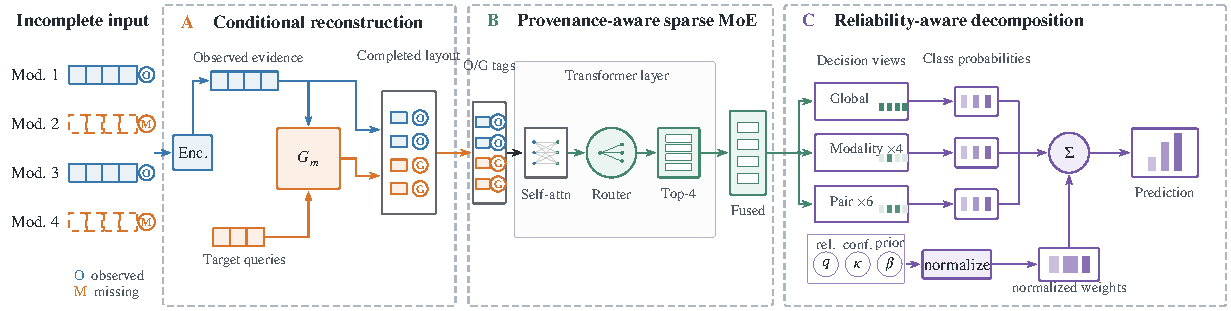
\includegraphics[width=\textwidth]{CERD_framework.pdf}
  \caption{CERD reconstructs unavailable modality tokens from observed subject context, preserves observed/generated provenance through sparse expert fusion, and combines multigranular branch predictions using normalized reliability-aware weights.}
  \label{fig:CERD}
\end{figure*}

\subsection{Conditional Evidence Reconstruction}
\label{sec:reconstruction}

A fixed missing-modality token assigns the same surrogate representation to every subject with the same availability pattern, so it cannot reflect differences in their observed evidence. CERD instead reconstructs each missing target conditionally from the current subject's available modalities. During training, a non-empty proper subset \(\mathcal S_n\subsetneq\mathcal O_n\) is sampled as context and \(\mathcal T_n=\mathcal O_n\setminus\mathcal S_n\) supplies reconstruction targets. Context modalities are independently dropped and the draw is repaired when necessary so that both \(\mathcal S_n\) and \(\mathcal T_n\) remain non-empty. This stochastic observed-subset construction exposes each generator to both rich and sparse contexts rather than only leave-one-modality-out cases.

For a reconstruction target \(m\in\mathcal T_n\), we first collect the context tokens in \(\mathbf Z_n^{\mathcal S}\). A target-specific generator then uses \(P\) learned queries \(\mathbf Q_m\) to retrieve the evidence needed for modality \(m\):
\begin{equation}
\begin{aligned}
\mathbf Z_n^{\mathcal S}
  &=\operatorname{Concat}_{j\in\mathcal S_n}\mathbf Z_n^j,\\
\widehat{\mathbf Z}_n^m
  &=G_m\!\left(\mathbf Q_m,\mathbf Z_n^{\mathcal S}\right).
\end{aligned}
\label{eq:generator}
\end{equation}
The generator applies cross-attention followed by feed-forward refinement. Its refined query sequence \(\mathbf U_n^m\) passes through a channel gate:
\begin{equation}
\widehat{\mathbf Z}_n^m
=\mathbf U_n^m\odot
\sigma\!\left(W_m^g\mathbf U_n^m+\mathbf b_m^g\right).
\label{eq:channel_gate}
\end{equation}
The gate suppresses query responses unsupported by the current context. At inference, all observed modalities form \(\mathbf Z_n^{\mathcal S}\), and generators are invoked only for missing targets. Thus, subjects with the same missing pattern can receive different reconstructions whenever their observed evidence differs.

Reconstruction is supervised at the pooled and token levels. Let \(\overline{\mathbf Z}\) denote token averaging, \(R_m\) a target-specific projector, \(\operatorname{LN}\) token-wise layer normalization, and \(\operatorname{sg}\) stop-gradient. For target \((n,m)\),
\begin{equation}
\begin{aligned}
\ell_{\mathrm{pool}}^{n,m}
 &=1-\cos\!\left(R_m(\overline{\widehat{\mathbf Z}}_n^m),
 \operatorname{sg}[R_m(\overline{\mathbf Z}_n^m)]\right),\\
\ell_{\mathrm{tok}}^{n,m}
 &=\operatorname{SmoothL1}\!\left(
 \operatorname{LN}(\widehat{\mathbf Z}_n^m),
 \operatorname{sg}[\operatorname{LN}(\mathbf Z_n^m)]\right).
\end{aligned}
\label{eq:reconstruction_terms}
\end{equation}
For a mini-batch \(\mathcal N\), these target losses are averaged as
\begin{equation}
\begin{aligned}
N_{\mathrm{rec}}
  &=\sum_{n\in\mathcal N}|\mathcal T_n|,\\
\mathcal L_{\mathrm{rec}}
  &=\frac{1}{N_{\mathrm{rec}}}
    \sum_{n\in\mathcal N}\sum_{m\in\mathcal T_n}
    \left(\ell_{\mathrm{pool}}^{n,m}
    +\lambda_{\mathrm{tok}}\ell_{\mathrm{tok}}^{n,m}\right).
\end{aligned}
\label{eq:reconstruction_loss}
\end{equation}
The pooled term preserves subject-level semantic direction, whereas the token term preserves the ordered slot structure. Stop-gradient fixes the encoded target while the generator learns to approach it. One generator is reused for every context of target \(m\): \(\mathbf Q_m\) specifies the target, while \(\mathbf Z_n^{\mathcal S}\) specifies the subject and available evidence. CERD therefore avoids a separate generator for every missingness pattern.

The two reconstruction levels constrain complementary failure modes. Pooled alignment alone can preserve a subject-level mean while losing slot organization, whereas token alignment alone can reproduce local structure without retaining the target's semantic direction. Their joint use makes generated tokens compatible with the fixed fusion layout at both resolutions.

\subsection{Provenance-Aware Sparse MoE Fusion}
\label{sec:sparse_moe}

Reconstruction supplies a complete latent layout, but reconstructed information should not be indistinguishable from an observed measurement. Before fusion, CERD therefore adds an observed or generated provenance embedding:
\begin{equation}
\widetilde{\mathbf Z}_n^m=
\begin{cases}
\mathbf Z_n^m+\mathbf e^{\mathrm{obs}}, & o_n^m=1,\\
\widehat{\mathbf Z}_n^m+\mathbf e^{\mathrm{gen}}, & o_n^m=0.
\end{cases}
\label{eq:source_embedding}
\end{equation}
These embeddings retain token origin while keeping all modalities in the same latent space.

The marked tokens are concatenated and processed by global self-attention. The Transformer feed-forward block is replaced by a sparse MoE layer. For token \(\mathbf h\), router \(\mathbf g\) defines the active expert set \(\mathcal A(\mathbf h)\), after which only those expert outputs are combined:
\begin{equation}
\begin{aligned}
\mathcal A(\mathbf h)&=\operatorname{TopK}(\mathbf g(\mathbf h),k),\\
\operatorname{MoE}(\mathbf h)
  &=\sum_{e\in\mathcal A(\mathbf h)}
    \pi_e(\mathbf h)F_e(\mathbf h).
\end{aligned}
\label{eq:sparse_moe}
\end{equation}
Here, \(F_e\) is expert \(e\), and \(\pi_e\) is its softmax weight within \(\mathcal A(\mathbf h)\). Because provenance is added before routing, expert selection can respond to modality content and observed--generated status. A load-balancing term promotes utilization of the expert pool. The fused sequence is finally separated by modality and pooled into context-enriched features \(\{\mathbf f_n^m\}_{m=1}^{M}\).

The attention and expert stages have complementary roles. Global self-attention communicates evidence across every modality position, whereas sparse feed-forward experts specialize the transformation applied to each resulting token. The router therefore adapts computation to both the subject and the observed--generated composition without creating a separate network for every missingness pattern. With \(M=4\) and \(P=16\), the shared sequence contains \(64\) tokens; only \(k=4\) of the \(16\) experts are active for each token. The MoE remains a shared representation backbone, and all subsequent diagnostic branches reuse its pooled modality features.

Routing follows self-attention, so expert assignments are computed from tokens that already encode whole-subject context rather than isolated unimodal features. Sparse specialization therefore refines cross-modal evidence while preserving one common modality layout; it does not partition the sources into independent processing streams.

\subsection{Reliability-Aware Evidence Decomposition}
\label{sec:evidence_fusion}

A single readout compresses the fused state into one decision view. CERD instead uses three readout granularities. Let \(0\) denote the global branch, \(m\in\mathcal M\) a modality-centered branch, and \((i,j)\in\mathcal P=\{(i,j):i<j\}\) a pair-centered branch. The complete branch set is \(\mathcal B=\{0\}\cup\mathcal M\cup\mathcal P\), and every branch produces a class-probability vector \(\mathbf p_n^b\). Because the readouts follow global attention and sparse experts, they are anchored to particular modality positions but retain cross-modal context. A pair branch receives
\begin{equation}
\mathbf u_n^{(i,j)}=
\left[\mathbf f_n^i;\mathbf f_n^j;
\mathbf f_n^i\odot\mathbf f_n^j;
|\mathbf f_n^i-\mathbf f_n^j|\right],
\label{eq:pair_feature}
\end{equation}
which represents agreement and discrepancy between its two anchors. With four modalities, \(\mathcal B\) contains one global, four modality-centered, and six pair-centered heads.

CERD then separates learned input reliability from predictive confidence. Let \(a_m\) be a small modality-specific reliability head. Because every missing target is generated from at least one observed source, modality reliability has two cases:
\begin{equation}
r_n^m=
\begin{cases}
1, & o_n^m=1,\\
\sigma\!\left(a_m(\mathbf f_n^m)\right), & o_n^m=0.
\end{cases}
\label{eq:modality_reliability}
\end{equation}
Observed evidence establishes the reference value, while generated evidence receives a subject-dependent score in \((0,1)\). Since \(r_n^m\) is optimized through the prediction objective, it quantifies task-specific predictive trust. The raw scores are estimated independently; normalization is applied when branches compete for decision weight and when cohort-level shares are visualized.

Branch reliability is then obtained directly from the modalities anchoring each readout:
\begin{equation}
q_n^b=
\begin{cases}
\displaystyle \frac{1}{M}\sum_{m=1}^{M}r_n^m, & b=0,\\[4pt]
r_n^m, & b=m,\\[2pt]
\sqrt{r_n^i r_n^j}, & b=(i,j).
\end{cases}
\label{eq:branch_reliability}
\end{equation}
The global mean remains on the scale of one reliability score, while the geometric mean requires support from both pair anchors. Predictive confidence is measured independently from the entropy \(H\) of the \(C\)-class branch distribution:
\begin{equation}
\kappa_n^b=\max\!\left(
1-\frac{H(\operatorname{sg}[\mathbf p_n^b])}{\log C},
\epsilon\right).
\label{eq:evidence_confidence}
\end{equation}
This score measures distributional concentration and is used to compare decision views~\cite{guo2017calibration,lakshminarayanan2017deepensembles,ovadia2019uncertainty}.

Because every modality position is either observed or conditionally generated, all decision views are evaluated. Original availability enters through provenance and Eq.~\eqref{eq:modality_reliability}. A learned scalar \(\beta_b\) supplies a prior for branch \(b\). The unnormalized evidence score, normalized branch weight, and final prediction are
\begin{equation}
\begin{aligned}
s_n^b&=(q_n^b+\epsilon)(\kappa_n^b+\epsilon)e^{\beta_b},\\
w_n^b&=\frac{s_n^b}{\sum_{b'\in\mathcal B}s_n^{b'}},\\
\mathbf p_n&=\sum_{b\in\mathcal B}w_n^b\mathbf p_n^b.
\end{aligned}
\label{eq:final_prediction}
\end{equation}
Thus, reliability \(q_n^b\), confidence \(\kappa_n^b\), and prior \(\beta_b\) have separate roles before normalization. The stored \(\mathbf p_n^b\) and \(w_n^b\) are forward-pass quantities, and their weighted sum exactly reproduces \(\mathbf p_n\).

Reliability and confidence serve distinct roles. A generated branch may be sharply peaked yet weakly supported by its inferred input; an observed view may be reliable but class-ambiguous. Their product requires both source support and discriminative concentration, while the branch prior captures stable utility without replacing subject-dependent variation.

For visualization, branch weights are summarized at the modality level. A modality-centered weight is assigned to its anchor, a modality-pair-centered weight is divided equally between its two anchors, and the global weight is distributed uniformly:
\begin{equation}
d_n^m=w_n^m+
\frac{1}{2}\sum_{j\ne m}w_n^{(m,j)}
+\frac{w_n^0}{M}.
\label{eq:modality_weight}
\end{equation}
The resulting modality decision allocation is a descriptive summary of the model decision, rather than an additional prediction mechanism.

\subsection{Training Objective}
\label{sec:objective}

CERD is trained end to end with five losses, each attached to a defined part of the method chain:
\begin{equation}
\mathcal L=
\mathcal L_{\mathrm{cls}}
+\lambda_b\mathcal L_{\mathrm{branch}}
+\lambda_r\mathcal L_{\mathrm{rec}}
+\lambda_g\mathcal L_{\mathrm{balance}}
+\mathcal L_{\mathrm{rob}}.
\label{eq:total_objective}
\end{equation}
Here, \(\mathcal L_{\mathrm{cls}}=|\mathcal N|^{-1}\sum_{n\in\mathcal N}\operatorname{CE}(y_n,\mathbf p_n)\) supervises the fused probability, and \(\mathcal L_{\mathrm{rec}}\) is defined in Eq.~\eqref{eq:reconstruction_loss}. Each branch is also trained directly. We first normalize its stopped reliability within mini-batch \(\mathcal N\), then apply reliability-weighted cross-entropy:
\begin{equation}
\begin{aligned}
\alpha_n^b
  &=\frac{\operatorname{sg}[q_n^b]}
  {\sum_{u\in\mathcal N}\operatorname{sg}[q_u^b]+\epsilon},\\
\mathcal L_{\mathrm{branch}}
  &=\frac{1}{|\mathcal B|}\sum_{b\in\mathcal B}
    \sum_{n\in\mathcal N}\alpha_n^b
    \operatorname{CE}(y_n,\mathbf p_n^b).
\end{aligned}
\label{eq:branch_loss}
\end{equation}
This term supervises every readout independently of its current mixture weight. For sparse layer \(\ell\), let \(\mathbf I_\ell\) collect the router probability received by each expert and \(\mathbf L_\ell\) its assigned-token counts. The load loss \(\mathcal L_{\mathrm{balance}}=\sum_{\ell}[\operatorname{CV}^2(\mathbf I_\ell)+\operatorname{CV}^2(\mathbf L_\ell)]\) promotes balanced expert use.

Robustness is trained from a strict non-empty reduced view \(\widetilde{\mathcal O}_n\subset\mathcal O_n\). Let \(\mathbf p_n\) and \(\widetilde{\mathbf p}_n\) be the original- and reduced-view predictions. The batch-averaged robustness loss is
\begin{equation}
\begin{aligned}
\mathcal L_{\mathrm{rob}}
&=\frac{1}{|\mathcal N|}\sum_{n\in\mathcal N}\Big[
\lambda_d\operatorname{CE}(y_n,\widetilde{\mathbf p}_n)\\
&\quad+\lambda_{\mathrm{sd}}T^2\operatorname{KL}\!\left(
\operatorname{sg}[\mathbf p_n^{(T)}]\,\|\,\widetilde{\mathbf p}_n^{(T)}\right)\\
&\quad+\lambda_{\mathrm{mf}}\left[
\operatorname{CE}(y_n,\mathbf p_n)-
\operatorname{CE}(y_n,\widetilde{\mathbf p}_n)
\right]_+\Big].
\end{aligned}
\label{eq:robust_objective}
\end{equation}
Superscript \((T)\) denotes temperature-scaled probabilities. The three lines respectively train reduced-view classification, transfer the original-view class distribution, and preserve the advantage of richer evidence. Reduced-view training constrains the final decision across availability patterns, whereas stochastic reconstruction contexts provide target supervision to the generators.

These two subset constructions impose different invariances. Reconstruction holds out observed targets to learn cross-modal recovery, whereas reduced-view training perturbs availability at the prediction level and constrains the resulting class distribution. Their combination couples target recovery to stable decisions rather than optimizing reconstruction and robustness as separate objectives.

\subsection{Inference and Computational Structure}
\label{sec:inference}

At inference, CERD first encodes the observed sources and conditionally generates only the missing targets. All modality positions then enter the provenance-aware backbone in a fixed \(MP\)-token layout. Sparse routing activates \(k\) feed-forward experts per token, while the attention path and parameters remain shared across availability patterns. The branch heads add only \(1+M+\binom{M}{2}\) shallow classifiers. Equation~\eqref{eq:final_prediction} then returns both the class probability and the exact weights that produced it. No reconstruction loss, reduced-view pass, or auxiliary explanation model is required during inference.

This organization has two practical consequences. First, the number of possible missingness patterns grows exponentially with \(M\), but CERD does not store a pattern-specific completion vector or prediction network. Target-specific generators are reused with any non-empty context, and sparse experts specialize at the token level. Second, the decision trace is available in the ordinary forward output: modality reliability describes the status of each supplied representation, branch probabilities describe the decisions supported at different granularities, and normalized weights state how those decisions were combined.

\section{Experiments}

\subsection{Datasets and Preprocessing}

\label{sec:datasets}

\noindent\textbf{ABCD.}
The ABCD Study characterizes adolescent brain, cognitive, behavioral, and health development~\cite{garavan2018abcd}. We derive three mutually exclusive groups from the baseline parent K-SADS ADHD assessment: (i)~a strict low-symptom comparator with no current, past, partial-remission, or unspecified ADHD and at most three current symptoms in either nine-item domain; (ii)~full ADHD with predominantly inattentive presentation, defined by at least six inattentive but fewer than six hyperactive/impulsive symptoms; and (iii)~full ADHD with a diagnostic-threshold hyperactive/impulsive component, comprising hyperactive/impulsive and combined presentations. Current symptoms are used for a current full diagnosis and past symptoms for a past full diagnosis; partial-remission-only and unspecified cases are excluded. The family-disjoint cohort contains \(2{,}868\) participants, split into \(2{,}041/414/413\) for training/validation/testing. The corresponding class counts are \(913/442/686\), \(170/94/150\), and \(187/99/127\).

ABCD predictors form four model modalities. Imaging (785 variables) concatenates rs-fMRI network connectivity and regional variance, regional contrast estimates from SST, emotional n-back, and MID task-fMRI, regional T1-weighted gray matter intensity, and DTI-derived FA. Genetics comprises 1,178 directly encoded SNP dosages retained after training-set missingness, minor allele frequency, and LD pruning within 14 prespecified candidate-gene windows; no PCA, PRS, or ancestry components are used. The cognition and health group contains 90 NIH Toolbox, WISC, Little Man, RAVLT, sleep, and physical-activity variables. The behavior and environment group begins with 221 non-ADHD behavioral, family, neighborhood, socioeconomic, and address-linked exposure variables, of which 218 survive training-only screening.

\noindent\textbf{ADNI.}
The Alzheimer's Disease Neuroimaging Initiative (ADNI) is a multicenter longitudinal study of biomarkers for cognitive decline and Alzheimer's disease~\cite{ref_adni}. We classify participants as cognitively normal, mild cognitive impairment, or Alzheimer's disease. Its four modalities are 187 regional FreeSurfer structural-MRI measurements, 387,639 directly encoded SNPs, 4,189 clinical and cognitive variables, and 151 biospecimen measurements. The cohort contains \(2{,}116\) participants: \(1{,}480\) for training, \(318\) for validation, and \(318\) for testing. Their class counts are \(648/522/310\), \(139/112/67\), and \(139/112/67\), respectively. In both datasets, a subject is retained when at least one selected modality is available.

\label{sec:missingness_protocol}

\noindent\textbf{Missing-modality patterns.}
ADNI follows source-table availability: \(27.64\%\), \(28.62\%\), and \(31.13\%\) of the training, validation, and test participants are incomplete, respectively. Every incomplete ADNI participant lacks exactly one of the four modalities, and none is all-missing. For ABCD, a fixed label-independent mask augments source-table availability to approximately \(15\%\) incomplete participants per split. Among additionally masked complete cases, one, two, or three modalities are withheld in proportions \(0.72\), \(0.23\), and \(0.05\). The all-missing case is forbidden, and every method receives the same split-specific inputs. Table~\ref{tab:missingness_counts} gives the exact final counts.

\begin{center}
\begin{minipage}{0.96\columnwidth}
\refstepcounter{table}\label{tab:missingness_counts}
\small\textbf{Table \thetable:} Incomplete participants in the fixed splits; entries are \(n/N\) (\%).
\vspace{4pt}

\centering
\small
\setlength{\tabcolsep}{4pt}
\renewcommand{\arraystretch}{1.30}
\begin{tabular*}{\columnwidth}{@{\extracolsep{\fill}}lrr@{}}
\toprule
Split & ADNI, \(n/N\) (\%) & ABCD, \(n/N\) (\%) \\
\midrule
Training & 409/1480 (27.64) & 306/2041 (14.99) \\
Validation & 91/318 (28.62) & 62/414 (14.98) \\
Testing & 99/318 (31.13) & 62/413 (15.01) \\
\bottomrule
\end{tabular*}
\end{minipage}
\end{center}

\label{sec:preprocessing}

\noindent\textbf{Preprocessing.}
For ABCD, imaging and tabulated variables with excessive missingness or near-zero variance are removed, after which available entries are median-imputed and standardized using training statistics. Genetic selection is likewise frozen from training participants: SNPs exceeding 2\% missingness or below 1\% minor-allele frequency are removed, followed by LD pruning with a 50-SNP window, five-SNP step, and \(r^2=0.8\) threshold. The retained 0/1/2 dosages are median-imputed and standardized without PCA. For ADNI, modality tables are joined by PTID and repeated FreeSurfer exports are deduplicated by database update stamp. Regional structural measurements are mean-imputed and standardized, genotypes are mode-imputed and transformed to \([-1,1]\), and missing entries in clinical and biospecimen tables are filled by training-column means. In both cohorts, entry-level imputation is applied only within an available modality. A wholly unavailable modality remains masked and is reconstructed only by CERD. All preprocessing statistics and feature-selection decisions are estimated from the training split.

\subsection{Experimental Setup}
\label{sec:experimental_setup}

\noindent\textbf{Implementation details.}

\label{sec:implementation}

CERD uses \(P=16\) tokens per modality on ADNI and \(P=8\) on ABCD, hidden dimension \(D=128\), one fusion layer with four attention heads, \(16\) experts, and top-\(4\) routing. Each target generator contains two cross-attention layers. We use \((\lambda_b,\lambda_g)=(0.1,0.01)\), \((\lambda_d,\lambda_{\mathrm{sd}},\lambda_{\mathrm{mf}})=(0.1,0.15,0.1)\), \(T=2\), and \(\epsilon=10^{-3}\). The reconstruction coefficient is 1.0 on ADNI and 0.25 on ABCD. Models are optimized for at most 50 epochs with AdamW; learning rates are \(1.25\!\times\!10^{-4}\) and \(1.0\!\times\!10^{-4}\), respectively. The checkpoint with the highest validation macro-F1 is evaluated once on the test set. Results are arithmetic mean \(\pm\) sample standard deviation over seeds 0/1/2 for ADNI and 31/32/33 for ABCD; probabilities are never ensembled across seeds.

\label{sec:evaluation}

\noindent\textbf{Evaluation metrics.}
We report accuracy, macro-F1, and macro-AUROC. Accuracy measures overall decisions, and macro-F1 assigns equal importance to the three clinical groups. Macro-AUROC averages one-vs-rest class ranking independently of a single operating point. The experiments ask whether CERD improves prediction under heterogeneous missingness, whether each stage contributes, whether performance is retained for incomplete participants, and whether evidence allocation agrees with controlled modality interventions. ABCD comparisons use the same family-disjoint split and participant-level mask for every method, with training-split preprocessing throughout.

The incomplete stratum is reported separately because aggregate performance can conceal a model that succeeds mainly on complete participants. Strict removal then holds participant identity fixed and turns the descriptive allocation into a testable prediction: removing evidence assigned greater decision mass should produce the larger score change.

\subsection{Comparison with Baselines}
\label{sec:main_results}
\label{sec:protocol}

\noindent\textbf{Compared methods.}
We compare CERD with six representative methods for incomplete multimodal learning. Flex-MoE combines a missing-modality bank with sparse routing~\cite{ref_flexmoe}. I$^2$MoE models unique, redundant, and synergistic multimodal interactions~\cite{xin2025i2moe}, whereas MoE++-corrected introduces learned, zero, copy, and constant experts~\cite{jin2025moepp}. AnyMod uses modality queries and a task anchor to accommodate arbitrary input combinations~\cite{feng2024anymod}. We further include task-matched implementations inspired by AGDiC and ACADiff because their original formulations operate on different neuroimaging representations~\cite{li2025agdic,zhou2026acadiff}. All methods use the same participant splits, modality groups, missingness patterns, and evaluation metrics.

\begin{table}[t]
\centering
\caption{Comparison on ADNI (\%). AUC denotes macro-AUROC; the best values are boldfaced.}
\label{tab:adni_results}
\setlength{\tabcolsep}{3pt}
\renewcommand{\arraystretch}{1.08}
\small
\begin{tabular*}{\columnwidth}{@{\extracolsep{\fill}}lrrr@{}}
\toprule
\textbf{Method} & \textbf{Acc.} & \textbf{Macro-F1} & \textbf{AUC} \\
\midrule
Flex-MoE~\cite{ref_flexmoe}
& 62.26$\pm$1.09 & 60.62$\pm$2.12 & 77.75$\pm$1.03 \\
I$^2$MoE~\cite{xin2025i2moe}
& 64.05$\pm$2.27 & 61.83$\pm$1.89 & 79.35$\pm$1.63 \\
MoE++-corrected~\cite{jin2025moepp}
& 59.75$\pm$0.54 & 58.85$\pm$2.06 & 79.23$\pm$1.39 \\
AnyMod~\cite{feng2024anymod}
& 64.78$\pm$4.63 & 63.55$\pm$4.28 & 79.77$\pm$2.12 \\
AGDiC-inspired~\cite{li2025agdic}
& 58.60$\pm$3.36 & 56.54$\pm$2.38 & 75.10$\pm$1.36 \\
ACADiff-inspired~\cite{zhou2026acadiff}
& 55.87$\pm$0.48 & 52.14$\pm$1.20 & 71.10$\pm$1.24 \\
\textbf{CERD (Ours)}
& \textbf{65.72$\pm$1.09} & \textbf{64.56$\pm$2.09} & \textbf{81.07$\pm$0.55} \\
\bottomrule
\end{tabular*}
\end{table}

\noindent\textbf{Main results.}
Table~\ref{tab:adni_results} shows that CERD ranks first on all three ADNI metrics. Relative to the strongest competing entry in each column, its mean accuracy, macro-F1, and AUROC are higher by \(0.94\), \(1.01\), and \(1.30\) points, respectively. The concurrent gains in macro-F1 and AUROC indicate that the benefit is not confined to the majority diagnosis: CERD improves class-balanced decisions while preserving stronger one-vs-rest ranking.

\begin{table}[t]
\centering
\caption{Comparison on the family-disjoint ABCD ADHD-presentation task with approximately 15\% incomplete participants (\%). AUC denotes macro-AUROC.}
\label{tab:abcd_results}
\setlength{\tabcolsep}{3pt}
\renewcommand{\arraystretch}{1.08}
\small
\begin{tabular*}{\columnwidth}{@{\extracolsep{\fill}}lrrr@{}}
\toprule
\textbf{Method} & \textbf{Acc.} & \textbf{Macro-F1} & \textbf{AUC} \\
\midrule
Flex-MoE
& 57.71$\pm$1.14 & 50.07$\pm$1.03 & 72.58$\pm$1.25 \\
I$^2$MoE
& 55.29$\pm$1.33 & 49.12$\pm$1.20 & 73.38$\pm$1.05 \\
MoE++-corrected
& 57.06$\pm$0.98 & 48.54$\pm$0.78 & 73.44$\pm$1.65 \\
AnyMod
& 54.48$\pm$4.44 & 48.46$\pm$4.23 & 69.60$\pm$3.16 \\
AGDiC-inspired
& 54.80$\pm$0.92 & 48.58$\pm$0.99 & 70.70$\pm$0.75 \\
ACADiff-inspired
& 54.32$\pm$1.22 & 47.00$\pm$0.71 & 68.31$\pm$0.63 \\
\textbf{CERD (Ours)}
& \textbf{59.24$\pm$1.65} & \textbf{53.62$\pm$1.40} & \textbf{74.43$\pm$1.03} \\
\bottomrule
\end{tabular*}
\end{table}

On ABCD, CERD ranks first in every column of Table~\ref{tab:abcd_results}. Its margins over the strongest corresponding baselines are \(1.53\), \(3.55\), and \(0.99\) points in accuracy, macro-F1, and macro-AUROC. The largest gain occurs in macro-F1, which is consistent with the endpoint design: the two ADHD groups differ by whether the hyperactive/impulsive domain crosses the diagnostic threshold, instead of mixing historical course and remission states within one intermediate class. CERD therefore benefits most where equal treatment of the three clinically defined groups is required.

\begin{table}[t]
\centering
\caption{CERD performance across test availability strata (\%, mean $\pm$ SD).}
\label{tab:availability_strata}
\setlength{\tabcolsep}{2.2pt}
\renewcommand{\arraystretch}{1.08}
\scriptsize
\begin{tabular*}{\columnwidth}{@{\extracolsep{\fill}}llrrrr@{}}
\toprule
\textbf{Data} & \textbf{Input} & \(n\) & \textbf{Acc.} & \textbf{Macro-F1} & \textbf{AUC} \\
\midrule
ADNI & Complete & 219 & 65.45$\pm$1.47 & 64.65$\pm$1.44 & 80.99$\pm$0.87 \\
 & Incomplete & 99 & 66.33$\pm$2.92 & 62.86$\pm$4.08 & 82.35$\pm$1.30 \\
ABCD & Complete & 351 & 59.54$\pm$1.78 & 53.88$\pm$1.94 & 75.02$\pm$0.75 \\
 & Incomplete & 62 & 57.53$\pm$4.93 & 51.84$\pm$5.83 & 72.39$\pm$2.17 \\
\bottomrule
\end{tabular*}
\end{table}

Table~\ref{tab:availability_strata} shows that CERD remains operational for incomplete participants in both cohorts. On ABCD, incomplete cases remain within 2.02 accuracy points of complete cases, while the higher variance reflects the smaller 62-participant stratum. Because the strata contain different participants, they describe deployment conditions rather than a causal effect of missingness; the matched within-participant removals in Section~\ref{sec:decision_analysis} isolate modality dependence directly.

\subsection{Ablation Study}
\label{sec:ablation_results}

\noindent\textbf{Compared variants.}
Each control starts from the dataset's full configuration and removes one named mechanism. Conditional completion is bypassed; provenance embeddings are suppressed; the sparse expert feed-forward block is replaced by an aligned dense FFN; multigranular decomposition is reduced to the global head and its associated specialist losses are removed; or adaptive branch scores are replaced by a uniform simplex. Every variant is independently trained and validation-selected with the same three seeds as its main result.

\begin{table*}[t]
\centering
\caption{Component analysis on both datasets (\%, mean $\pm$ SD). Each ``w/o'' row changes only the named mechanism; the full configuration is boldfaced. AUC denotes macro-AUROC.}
\label{tab:component_ablation}
\setlength{\tabcolsep}{3.2pt}
\renewcommand{\arraystretch}{1.08}
\scriptsize
\begin{tabular*}{\textwidth}{@{\extracolsep{\fill}}lrrrrrr@{}}
\toprule
& \multicolumn{3}{c}{\textbf{ADNI}} & \multicolumn{3}{c}{\textbf{ABCD}} \\
\cmidrule(lr){2-4}\cmidrule(lr){5-7}
\textbf{Configuration} & \textbf{Acc.} & \textbf{Macro-F1} & \textbf{AUC} & \textbf{Acc.} & \textbf{Macro-F1} & \textbf{AUC} \\
\midrule
w/o Conditional Completion & 63.73$\pm$0.79 & 62.82$\pm$1.58 & 79.48$\pm$0.41 & 55.61$\pm$1.94 & 50.95$\pm$1.58 & 71.41$\pm$1.03 \\
w/o Provenance Embeddings & 63.52$\pm$1.57 & 63.41$\pm$1.95 & 80.50$\pm$0.70 & 59.16$\pm$1.85 & 53.42$\pm$1.58 & 74.44$\pm$1.03 \\
w/o Sparse MoE (Dense FFN) & 64.99$\pm$1.19 & 65.27$\pm$1.12 & 81.59$\pm$0.74 & 59.08$\pm$2.31 & 54.33$\pm$1.43 & 75.11$\pm$1.07 \\
w/o Multigranular Decomposition & 62.47$\pm$0.79 & 62.36$\pm$1.00 & 79.72$\pm$1.32 & 56.98$\pm$3.72 & 53.04$\pm$3.19 & 74.06$\pm$1.10 \\
w/o Reliability-aware Weights & 64.05$\pm$1.49 & 63.88$\pm$0.21 & 80.95$\pm$0.19 & 59.32$\pm$1.59 & 54.35$\pm$2.30 & 73.81$\pm$0.78 \\
\textbf{Full CERD} & \textbf{65.72$\pm$1.09} & \textbf{64.56$\pm$2.09} & \textbf{81.07$\pm$0.55} & \textbf{59.24$\pm$1.65} & \textbf{53.62$\pm$1.40} & \textbf{74.43$\pm$1.03} \\
\bottomrule
\end{tabular*}
\end{table*}

\noindent\textbf{Ablation results.}
Table~\ref{tab:component_ablation} identifies conditional completion as the most consistent component across endpoints. Bypassing it reduces all three ABCD metrics by 2.67--3.63 points and all ADNI metrics by 1.19--1.99 points, linking subject-conditioned recovery to both discrimination and ranking. Collapsing the multigranular stage to the global head lowers accuracy by 3.25 points on ADNI and 2.26 points on ABCD, showing that source-anchored and pair-anchored readouts recover decisions not retained by global pooling alone. Provenance has a smaller isolated effect on ABCD, while the dense and uniform controls trade accuracy against macro-averaged metrics. These trade-offs do not support a universal per-column gain; instead, full CERD is the only configuration that combines the strongest ADNI result with the highest ABCD accuracy among the component controls.

\subsection{Modality Contribution Analysis}
\label{sec:decision_analysis}

We characterize source use with two complementary quantities. First, Eq.~\eqref{eq:modality_weight} assigns every branch weight to its modality anchors, yielding a normalized allocation whose four entries sum to one for each participant. Second, strict leave-one-modality-out intervention is evaluated on the originally complete test subset: the selected input block is zeroed, marked unavailable, and excluded from conditional completion. This holds participant identity fixed and measures the change in the same trained model. All quantities are computed independently for each seed before arithmetic aggregation.

\begin{table}[t]
\centering
\caption{Normalized decision allocation and strict-removal decreases (percentage points, mean $\pm$ SD). Allocation is averaged over the full test cohort; metric decreases use originally complete participants.}
\label{tab:modality_contribution}
\setlength{\tabcolsep}{1.7pt}
\renewcommand{\arraystretch}{1.07}
\scriptsize
\begin{tabular*}{\columnwidth}{@{\extracolsep{\fill}}llrrrr@{}}
\toprule
\textbf{Data} & \textbf{Modality} & \textbf{Alloc.} & \textbf{$\Delta$Acc.} & \textbf{$\Delta$F1} & \textbf{$\Delta$AUC} \\
\midrule
ADNI & MRI & 23.67$\pm$1.77 & 43.07$\pm$1.47 & 52.46$\pm$1.44 & 21.51$\pm$5.62 \\
 & Genetics & 21.81$\pm$1.68 & 9.28$\pm$12.36 & 18.14$\pm$21.49 & 2.49$\pm$3.19 \\
 & Clinical & 28.16$\pm$0.52 & 6.70$\pm$4.34 & 9.61$\pm$7.26 & 1.98$\pm$1.72 \\
 & Biospecimen & 26.36$\pm$0.44 & 38.81$\pm$5.94 & 49.95$\pm$4.35 & 17.75$\pm$13.65 \\
\midrule
ABCD & Imaging & 24.38$\pm$1.14 & 6.74$\pm$7.81 & 5.08$\pm$5.56 & 0.97$\pm$2.63 \\
 & Genetics & 23.68$\pm$4.16 & 8.74$\pm$8.97 & 12.99$\pm$7.82 & 0.87$\pm$2.49 \\
 & Cog./health & 25.74$\pm$1.36 & 14.25$\pm$1.24 & 30.18$\pm$2.58 & 0.75$\pm$1.11 \\
 & Behav./env. & 26.19$\pm$3.38 & 15.29$\pm$1.94 & 33.25$\pm$2.29 & 15.20$\pm$2.12 \\
\bottomrule
\end{tabular*}
\end{table}

\begin{figure}[t]
\centering
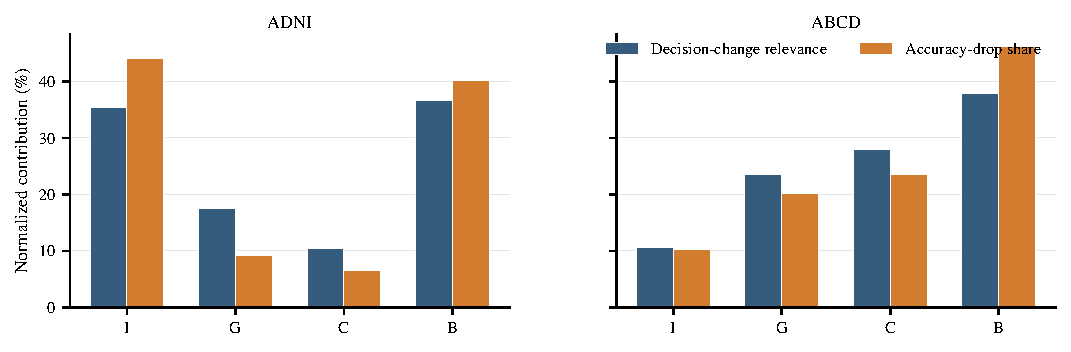
\includegraphics[width=0.98\columnwidth]{cerd_two_dataset_modality_drop_v1.pdf}
\caption{Accuracy decrease under strict modality removal. I, G, C, and B denote MRI, genetics, clinical, and biospecimen inputs on ADNI; on ABCD they denote imaging, genetics, cognition/health, and behavior/environment. Bars and error bars show the three-seed mean and sample standard deviation.}
\label{fig:two_dataset_modality_drop}
\end{figure}

Table~\ref{tab:modality_contribution} and Fig.~\ref{fig:two_dataset_modality_drop} reveal endpoint-specific dependence within a non-collapsed allocation profile. ADNI is most sensitive to MRI and biospecimen removal, consistent with complementary structural and molecular evidence for neurodegenerative status. For ABCD presentation classification, cognition/health and behavior/environment produce the largest accuracy and macro-F1 decreases, and behavior/environment also causes the largest AUROC decrease. This ordering is coherent with an endpoint defined by symptom presentation: cognitive functioning and behavioral context are more directly coupled to the class boundary, while imaging and SNP evidence remains complementary and more seed-dependent. Allocation nevertheless stays distributed across all four sources, indicating multiple active evidence routes rather than a single-source gate.

\section{Discussion}
\label{sec:discussion}

\noindent\textbf{Coupling completion with controlled trust.}
CERD leads all three reported metrics on both datasets while operating on naturally and synthetically incomplete inputs. Conditional queries recover target-specific evidence, provenance exposes its origin to attention and routing, and reliability determines its decision influence. Conditional completion has the clearest isolated effect: removing it lowers every metric on both cohorts. Provenance produces a larger gain on ADNI than ABCD, indicating that its marginal value depends on how strongly the endpoint uses generated evidence.

\noindent\textbf{Sparse specialization of completed evidence.}
Because provenance precedes routing, the sparse MoE specializes transformations using semantic content, modality position, and evidence origin. The dense-FFN control retains reconstruction and decomposition, thereby isolating token-dependent expert computation. Sparse routing raises accuracy on both datasets, whereas the dense block improves several macro-averaged cells. This trade-off indicates that expert specialization principally sharpens the final class decision rather than uniformly shifting every ranking statistic.

\noindent\textbf{Why multigranular decomposition matters.}
Reducing CERD to its global head produces the largest ADNI accuracy decline and lowers accuracy and AUROC on ABCD. The anchored branches are not isolated unimodal or bimodal encoders: every \(\mathbf f_n^m\) already contains cross-modal context. Instead, modality and pair anchors expose source-centered and agreement--discrepancy views of that shared state. Their benefit across two endpoints shows that decision granularity adds information beyond a single pooled representation.

\noindent\textbf{Prediction consistency.}
The modality audit locates this evidence at the endpoint level. ADNI depends most on structural MRI and biospecimens, whereas ABCD ADHD presentation is most sensitive to cognition/health and behavior/environment. Normalized allocations nevertheless remain distributed across all four sources. CERD thus preserves complementary evidence routes while allowing the biological endpoint to determine their predictive dependence.

\section{Conclusion}

CERD combines conditional token recovery, sparse provenance-aware expert fusion, and reliability-based evidence decomposition. It gives the strongest result across all reported metrics on both ADNI and ABCD among matched baselines. Across cohorts, controls isolate completion, provenance, multigranular readout, and endpoint-specific modality dependence. Branch probabilities and normalized weights directly compose both the prediction and its evidence allocation.

\clearpage
% Preserve the CAS reference style while using a slightly larger, more
% readable bibliography setting for the final two-column layout.
\renewcommand{\bibfont}{\fontsize{8.8pt}{10.92pt}\selectfont}
\setlength{\bibsep}{0.15pt}
\bibliographystyle{cas-model2-names}
\bibliography{cas-refs}

\end{document}
